\documentclass[a4paper]{article}
\usepackage[14pt]{extsizes} 
\usepackage[T2A]{fontenc}
\usepackage[utf8]{inputenc}
\usepackage{natbib}
\usepackage{graphicx}
\usepackage{amsmath}
\usepackage[english]{babel}
\usepackage{fontspec}
\usepackage{amsmath,amsfonts,amssymb,amsthm,mathtools,mathrsfs}
\usepackage{icomma}
\usepackage{fullpage}
\usepackage{ulem}
\usepackage{eufrak}
\usepackage{setspace}
\usepackage{listings}
\usepackage{indentfirst}
\usepackage[left=2cm,right=1.5cm,top=2cm,bottom=2cm]{geometry}
\usepackage{xcolor}
\usepackage{float}
\usepackage{csquotes}

\setmainfont[Ligatures={TeX,Historic}]{Times New Roman}
\setlength{\parindent}{5ex}
\setlength{\parskip}{1em}
\renewcommand{\baselinestretch}{1}

\graphicspath{{images/}}

\definecolor{buzzlightyear}{HTML}{8757A5}
\definecolor{grass}{HTML}{738D06}
\definecolor{literal}{HTML}{F18A2B}
\definecolor{commentcolor}{HTML}{8E908B}

\lstdefinestyle{habrstyle}{
    backgroundcolor=\color{white},   
    commentstyle=\color{commentcolor},
    keywordstyle=\bfseries\color{buzzlightyear},
    numberstyle=\tiny\color{commentcolor},
    stringstyle=\color{grass},
    basicstyle=\ttfamily\footnotesize,
    breakatwhitespace=false,         
    breaklines=true,                 
    captionpos=b,                    
    keepspaces=true,                 
    numbers=left,                    
    numbersep=5pt,                  
    showspaces=false,                
    showstringspaces=false,
    showtabs=false,                  
    tabsize=4
}

\lstset{style=habrstyle}

\begin{document}

    % FIRST PAGE
    \begin{center}
        \begin{center}
        \hfill \break
        \normalsize{Санкт-Петербургский государственный политехнический}\\
        \normalsize{университет Петра Великого}\\
        \hfill \break
        \normalsize{\textbf{Высшая школа интеллектуальных систем и}}\\ 
        \normalsize{\textbf{суперкомпьютерных технологий}}\\ 
        \hfill \break
        \hfill \break
        \hfill \break
        \normalsize{Лабораторная работа}\\
        \hfill \break
        \hfill \break
        \normalsize{\LARGE Модуляция и выборка (квантование)}\\
        \end{center}
        \hfill \break
        \hfill \break
        \hfill \break
        \hfill \break
        \hfill \break
        \hfill \break
        \hfill \break
        \hfill \break
        \hfill \break
        \hfill \break
        \begin{flushright}
            \normalsize{Работу выполнил студент}\\
            \normalsize{3-го курса, группа 3530901/80201}\\
            \normalsize{Сахибгареев Рамис Ринатович}\\
            \hfill \break
            \normalsize{Преподаватель:}\\
            \normalsize{Богач Наталья Владимировна}\\
        \end{flushright}
        \hfill \break
        \hfill \break
        \hfill \break
        \hfill \break
        \begin{center} Санкт-Петербург 2021 \end{center}
        \thispagestyle{empty}
    \end{center}
    % FIRST PAGE [END]
    
    \newpage
        \tableofcontents
    
    \newpage
         \listoffigures
    
    \newpage
         \lstlistoflistings   
     
    % START START START START START
    \newpage
        \section{Part 1: Research and execution of chap11}
        
        In this part we need to research and execute existing chap11.ipynb file, that contains information about amplitude modulation, convolution with impulses, sampling and sinc interpolation.
        
        \begin{figure}[H]
            \centering
            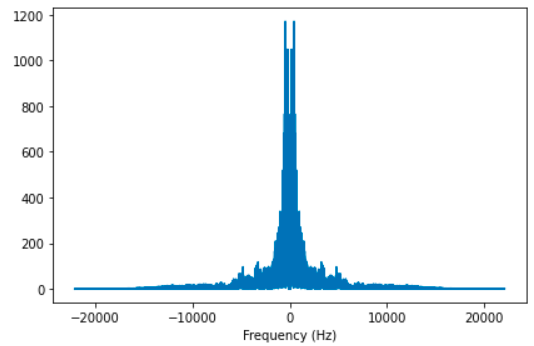
\includegraphics[width=\textwidth]{img/p1_1.png}
            \caption{After padding}
            \label{fig:p1_2}
        \end{figure}
        
        \begin{figure}[H]
            \centering
            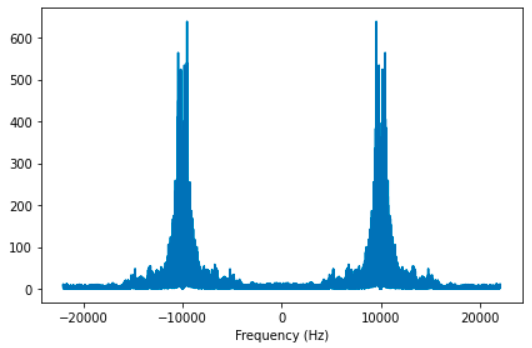
\includegraphics[width=\textwidth]{img/p1_2.png}
            \caption{Without padding}
            \label{fig:p1_2}
        \end{figure}
        
        \begin{figure}[H]
            \centering
            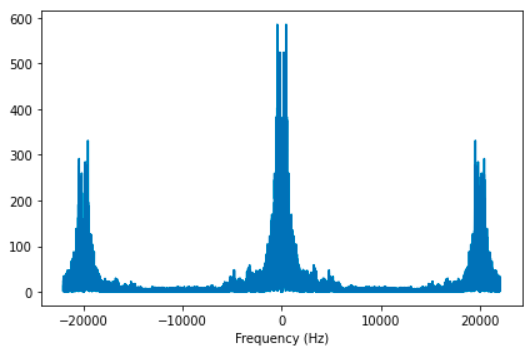
\includegraphics[width=\textwidth]{img/p1_3.png}
            \caption{Trying to apply convolution theorem on non periodic signal}
            \label{fig:p1_1}
        \end{figure}
        
        \begin{figure}[H]
            \centering
            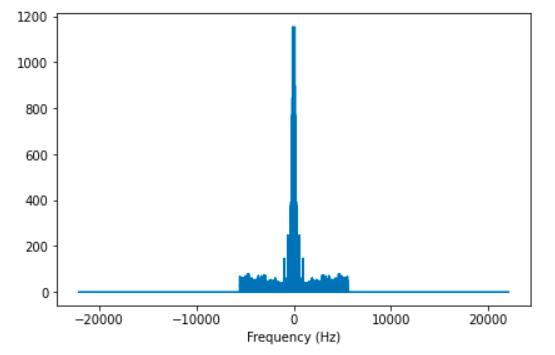
\includegraphics[width=\textwidth]{img/p1_4.png}
            \caption{After padding}
            \label{fig:p1_2}
        \end{figure}
        
        We can clearly see how aliasing effect appears while we are trying to use DFT with low frequency. It happens because of modulation, that splits the signal into the different parts around frequency of the signal. If this frequency is small, then resulting signals will overlap.
        
        \begin{figure}[H]
            \centering
            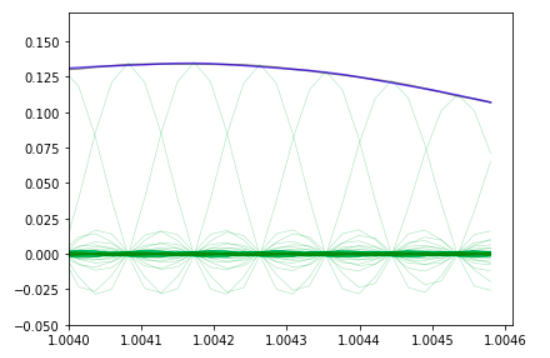
\includegraphics[width=\textwidth]{img/p1_5.png}
            \caption{After padding}
            \label{fig:p1_2}
        \end{figure}
        
        We can see, how box low pass filter spectrum looks. different sin signals are sums up resulting original wave.
        
    \newpage
        \section{Part 2: D/A and A/D | Digital Show and Tell}
    
        In this part we need to watch video about DC and AC transformations (https://www.youtube.com/watch?v=cIQ9IXSUzuM).
        
        After watching it we've learned, why do we use DFT, how transformation performed, why audio 44.1 KHz and \[2^16\] is enough for humans.
        
    \newpage
        \section{Part 3: Modulating the signal}

        In this part we need to try remove aliasing by applying low-pass filter before modulating and not after.
        
        \begin{lstlisting}[language=Python,caption=Reading the signal,label={lst:part1_2}]
    import numpy as np
    import matplotlib as plt
    from thinkdsp import *
    
    wave = read_wave('263868__kevcio__amen-break-a-160-bpm.wav')
    wave.normalize()
    wave.make_spectrum(full=True).plot()
    decorate(xlabel='Frequency (Hz)')
        \end{lstlisting}
        
        \begin{figure}[H]
            \centering
            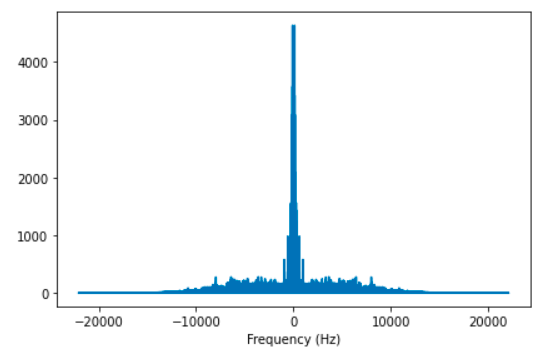
\includegraphics[width=\textwidth]{img/p2_1.png}
            \caption{Impulse's wave}
            \label{fig:part1_1_2}
        \end{figure}
        
        We can see, that signal has a lot of high frequency components, but they have low amplitude.
        
        
        \begin{lstlisting}[language=Python,caption=Reading the impulse,label={lst:part1_2}]
    spectrum = wave.make_spectrum(full=True)
    spectrum.low_pass(5000)
    wave = spectrum.make_wave()
    spectrum.plot()
    decorate(xlabel='Frequency (Hz)')
        \end{lstlisting}
        
        \begin{figure}[H]
            \centering
            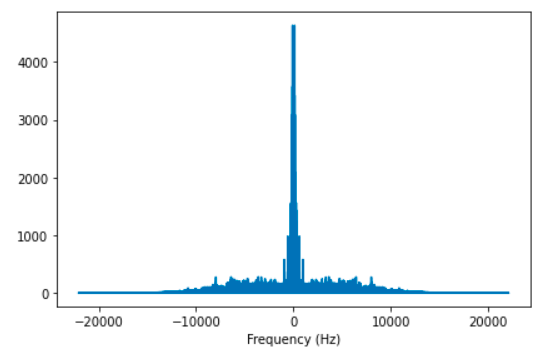
\includegraphics[width=\textwidth]{img/p2_1.png}
            \caption{Impulse's wave}
            \label{fig:part1_1_2}
        \end{figure}
        
        \begin{lstlisting}[language=Python,caption=Modulating the signal,label={lst:part1_2}]
    def sample(wave, factor):
        ys = np.zeros(len(wave))
        ys[::factor] = wave.ys[::factor]
        return Wave(ys, framerate=wave.framerate)
    sampled = sample(wave, 4)
    sampled.make_spectrum(full=True).plot()
    decorate(xlabel='Frequency (Hz)')
        \end{lstlisting}
        
        \begin{figure}[H]
            \centering
            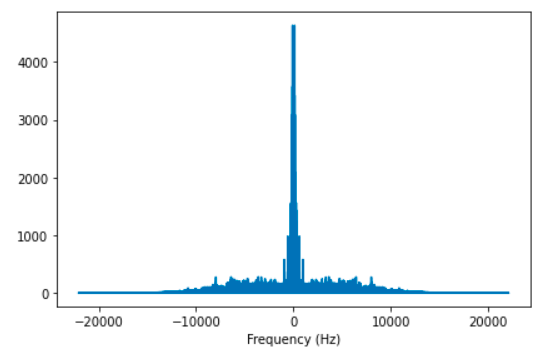
\includegraphics[width=\textwidth]{img/p2_1.png}
            \caption{Impulse's wave}
            \label{fig:part1_1_2}
        \end{figure}
        
        We can see, that no overlapping happened.
        
        
        \begin{lstlisting}[language=Python,caption=Getting modulated,label={lst:part1_2}]
    spectrum = sampled.make_spectrum(full=True)
    spectrum.low_pass(5512.5)
    sampled = spectrum.make_wave()
    spectrum.plot()
    decorate(xlabel='Frequency (Hz)')
        \end{lstlisting}
        
        \begin{figure}[H]
            \centering
            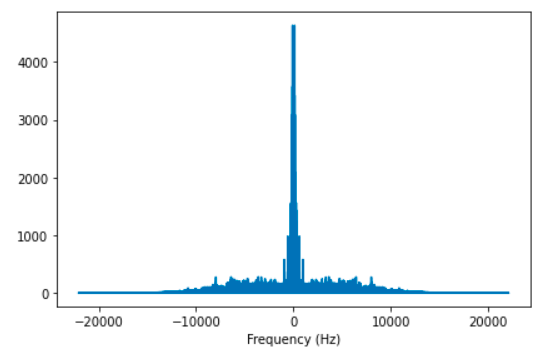
\includegraphics[width=\textwidth]{img/p2_1.png}
            \caption{Impulse's wave}
            \label{fig:part1_1_2}
        \end{figure}
        
        \begin{figure}[H]
            \centering
            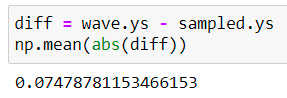
\includegraphics[width=\textwidth]{img/p2_5.png}
            \caption{Difference}
            \label{fig:part1_1_2}
        \end{figure}
        
        We can see, that the original and modulated signal has little difference.
            
    \newpage
        \section{Conclusion}
            We've learned, how amplitude modulation, convolution with impulses, samplingand sinc interpolation done and how we can use it for data transport. Also we've watched an video, that tells how and why DC and AC transformations performed. Finally we've tested a way how we can remove aliasing effect by applying a low-pass before modulation, not after.
     
\end{document}
